% !TeX spellcheck = de_DE
\documentclass[10pt,a4paper]{article}
\usepackage[latin1]{inputenc}
\usepackage{amsmath}
\usepackage{amsfonts}
\usepackage{amssymb}
\usepackage{graphicx}
\usepackage{hyperref}
\usepackage[paperheight=21cm,left=1cm,right=1cm]{geometry}
\pagestyle{empty}
\setlength\parindent{0pt}

\begin{document}

\section{Den playground auschecken}

RapidSVN starten

\begin{center}
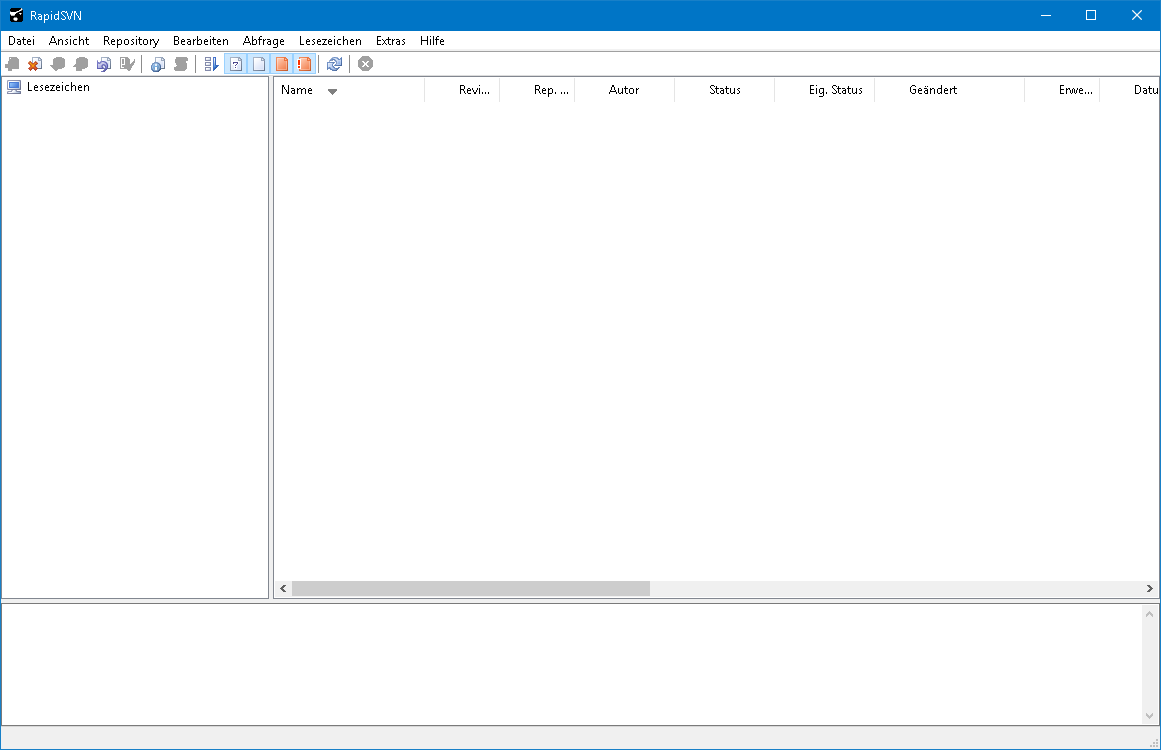
\includegraphics[width=\linewidth]{rapid1}
\end{center}

\clearpage

Repository $\Rightarrow$ Auschecken...

URL zum playground im Repository (\url{https://svn.informatik.uni-rostock.de/lehre/ip2019/playground/}) und Pfad f�r lokale Arbeitskopie (auf Laufwerk \texttt{R:}) eintragen

\begin{center}
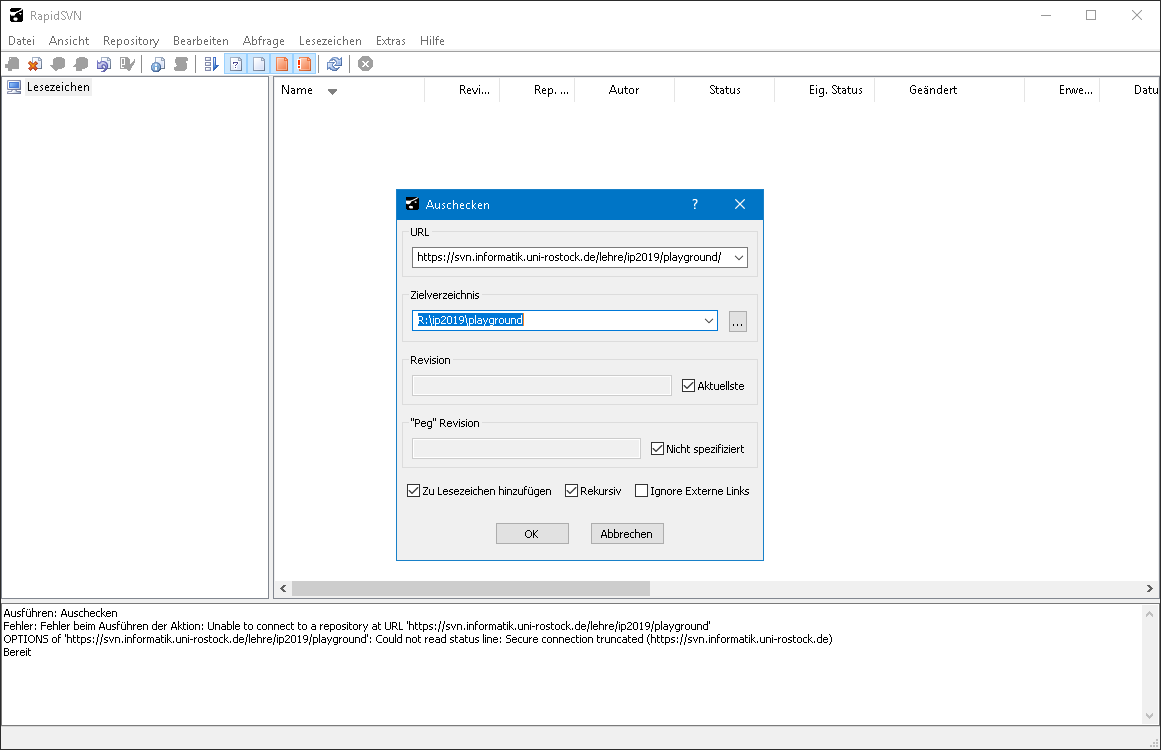
\includegraphics[width=\linewidth]{rapid4}
\end{center}

\clearpage

Ggf. Zertifikat akzeptieren.

\begin{center}
	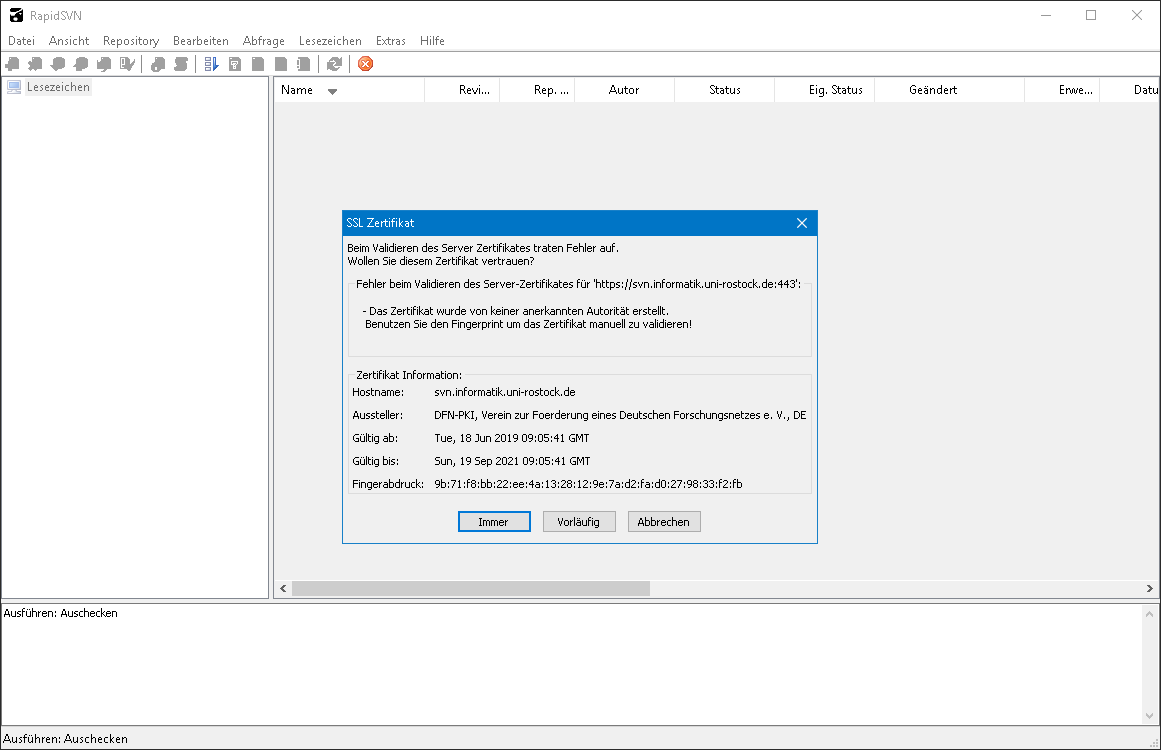
\includegraphics[width=\linewidth]{rapid3}
\end{center}

\clearpage

Authentifizieren mit ITMZ-Account...

\begin{center}
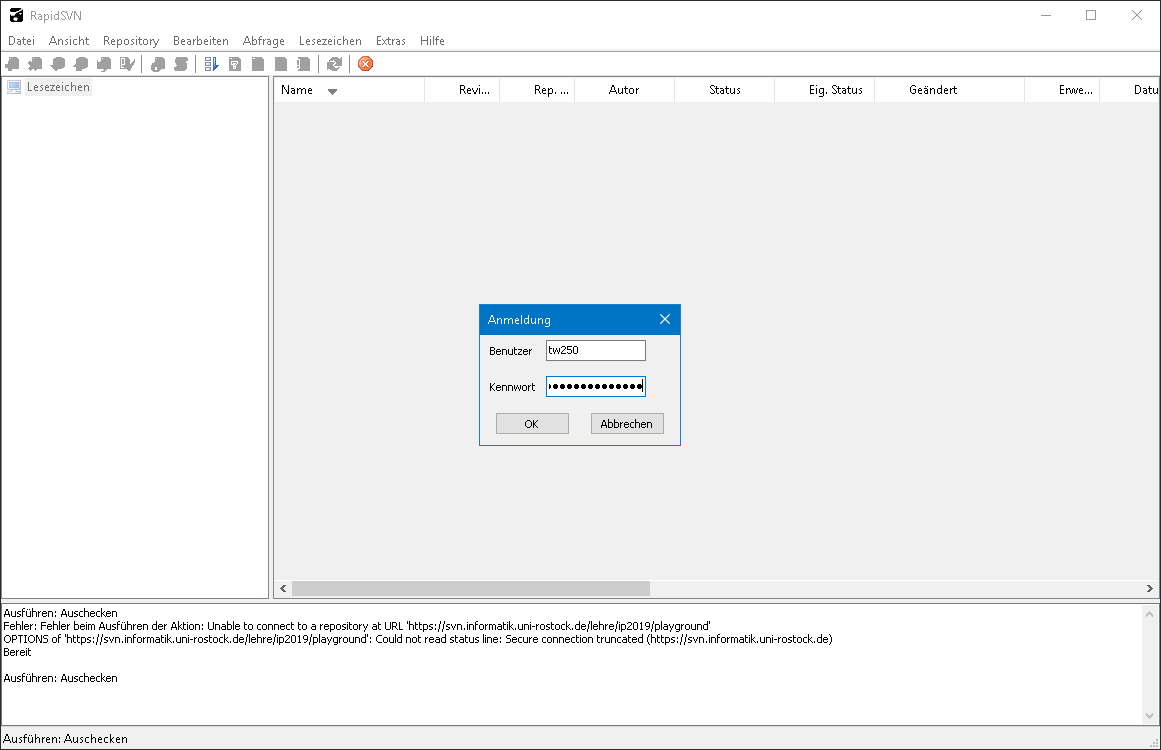
\includegraphics[width=\linewidth]{rapid6}
\end{center}

\clearpage

Fertig!

\begin{center}
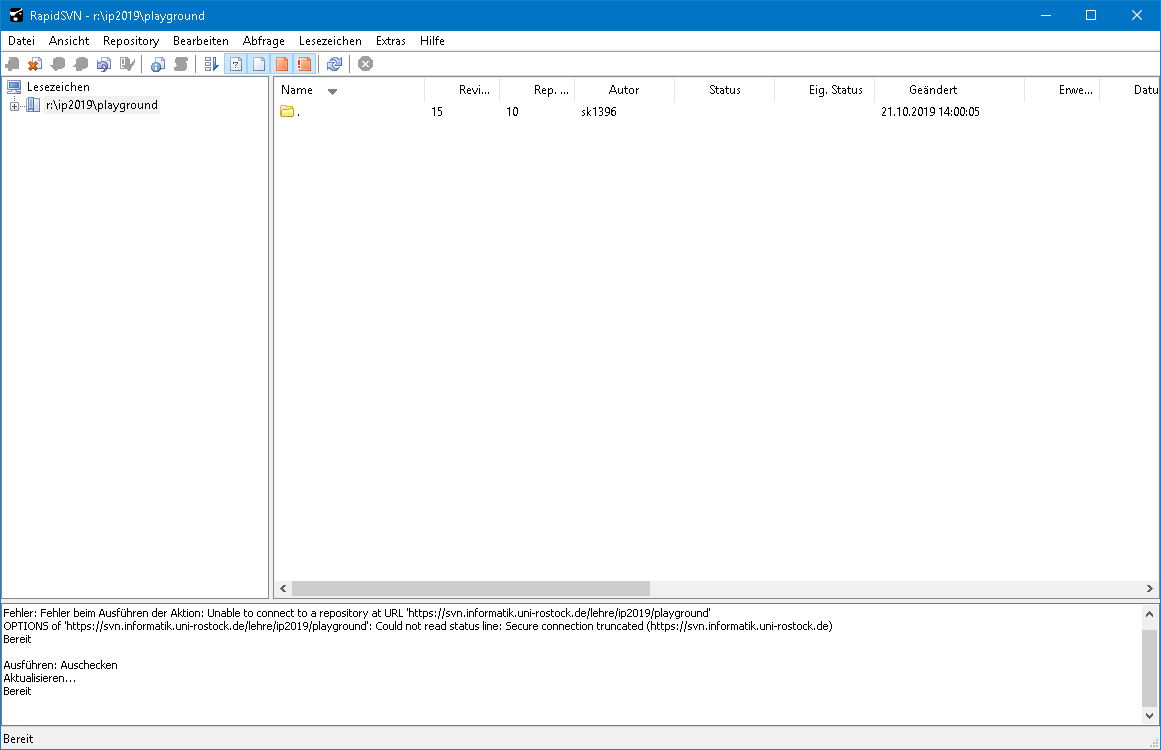
\includegraphics[width=\linewidth]{rapid7}
\end{center}

\clearpage

\section{Einen Ordner commiten}

Wir k�nnen im ausgecheckten Ordner einen Ordner anlegen.

\begin{center}
	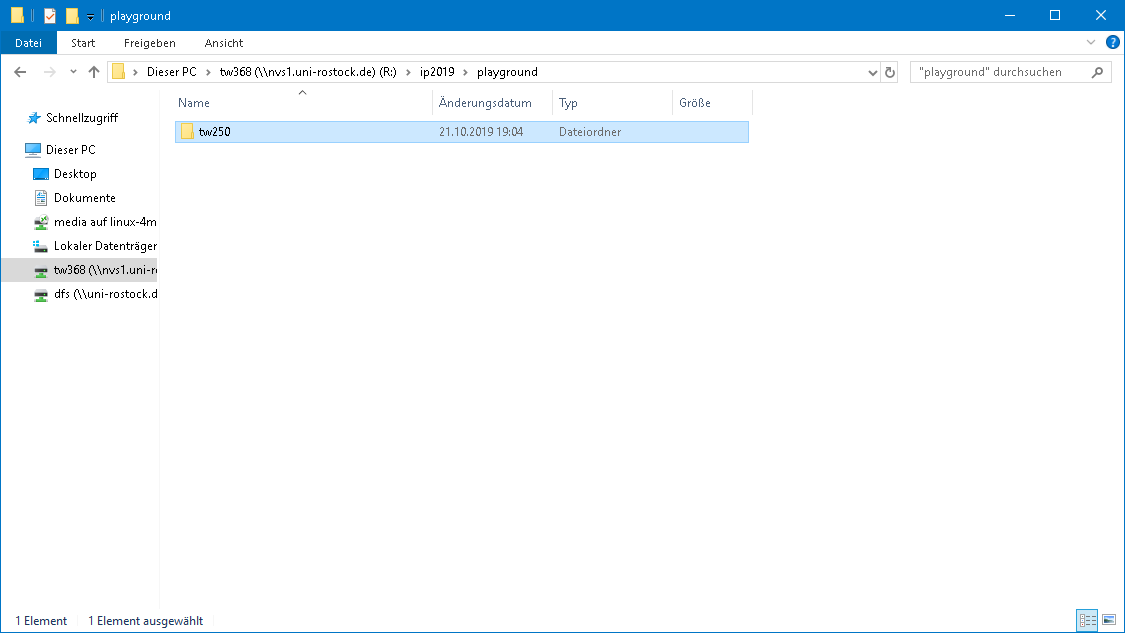
\includegraphics[width=\linewidth]{rapid8}
\end{center}

\clearpage

Ein Ordner, der in der Arbeitskopie angelegt wird, ist zun�chst unversioniert.

\begin{center}
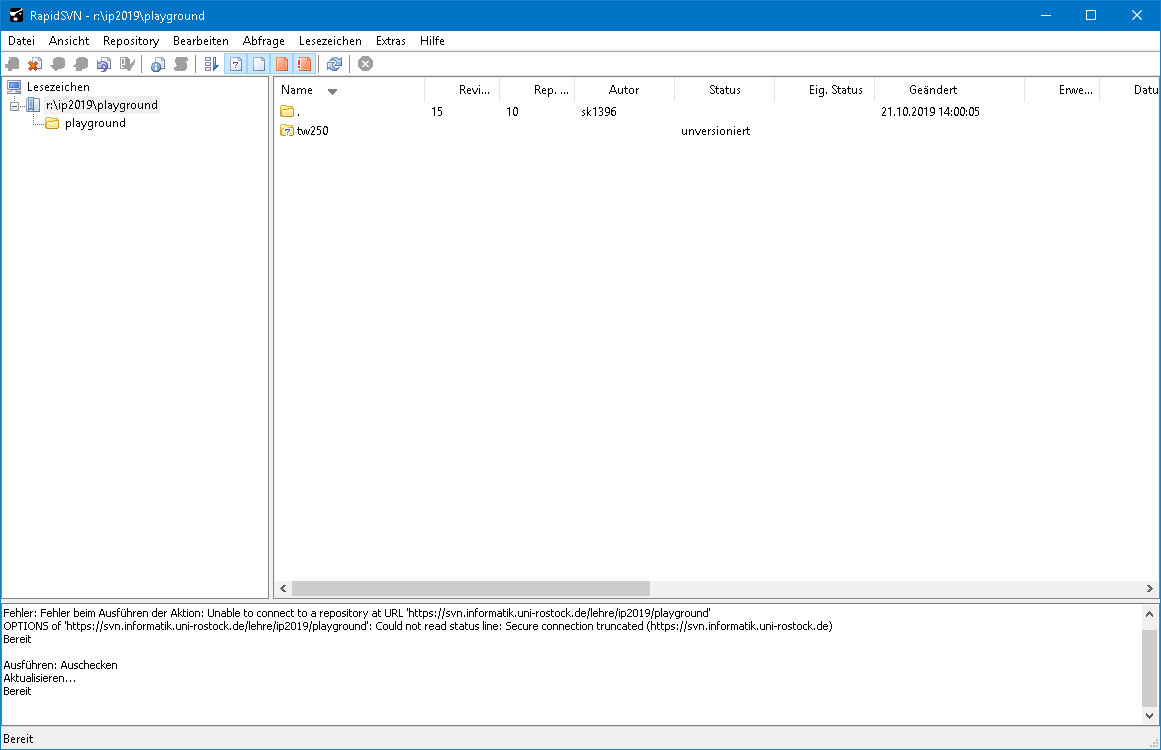
\includegraphics[width=\linewidth]{rapid9}
\end{center}

\clearpage

Wir f�gen ihn also dem Repository hinzu und stellen ihn damit unter Versionsverwaltung.

\begin{center}
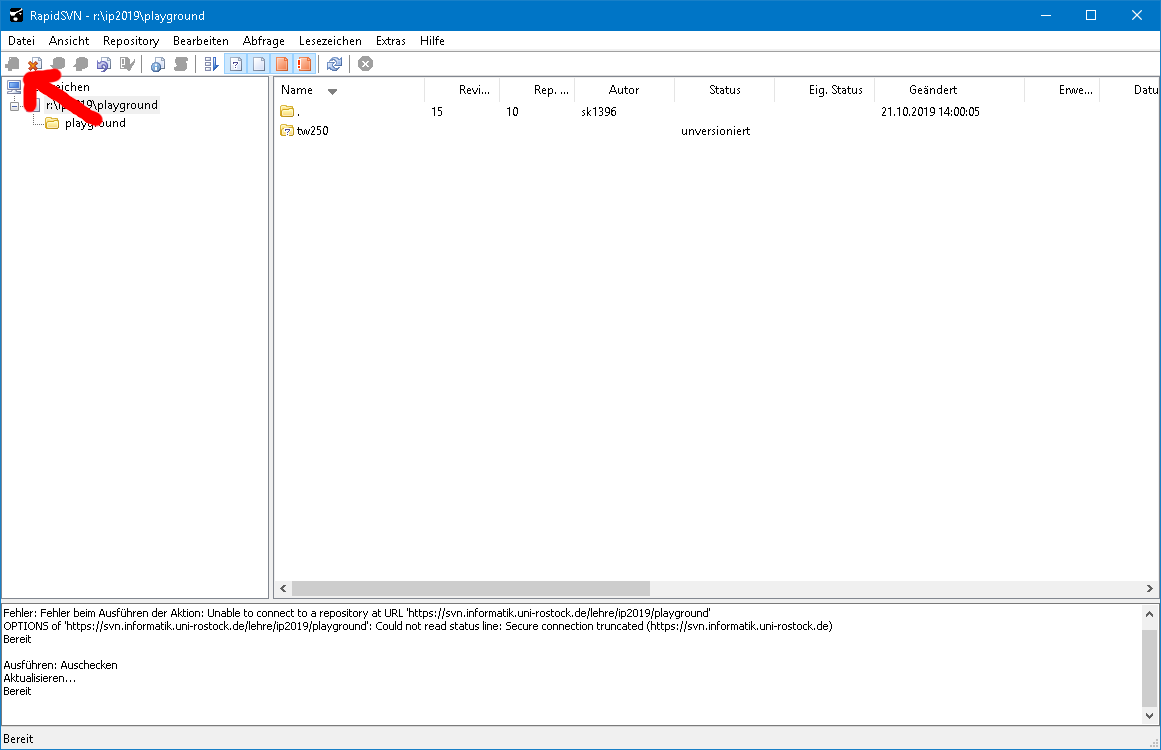
\includegraphics[width=\linewidth]{rapid9-2}
\end{center}

\clearpage

Nun k�nnen wir den hinzugef�gten Ordner commiten.

\begin{center}
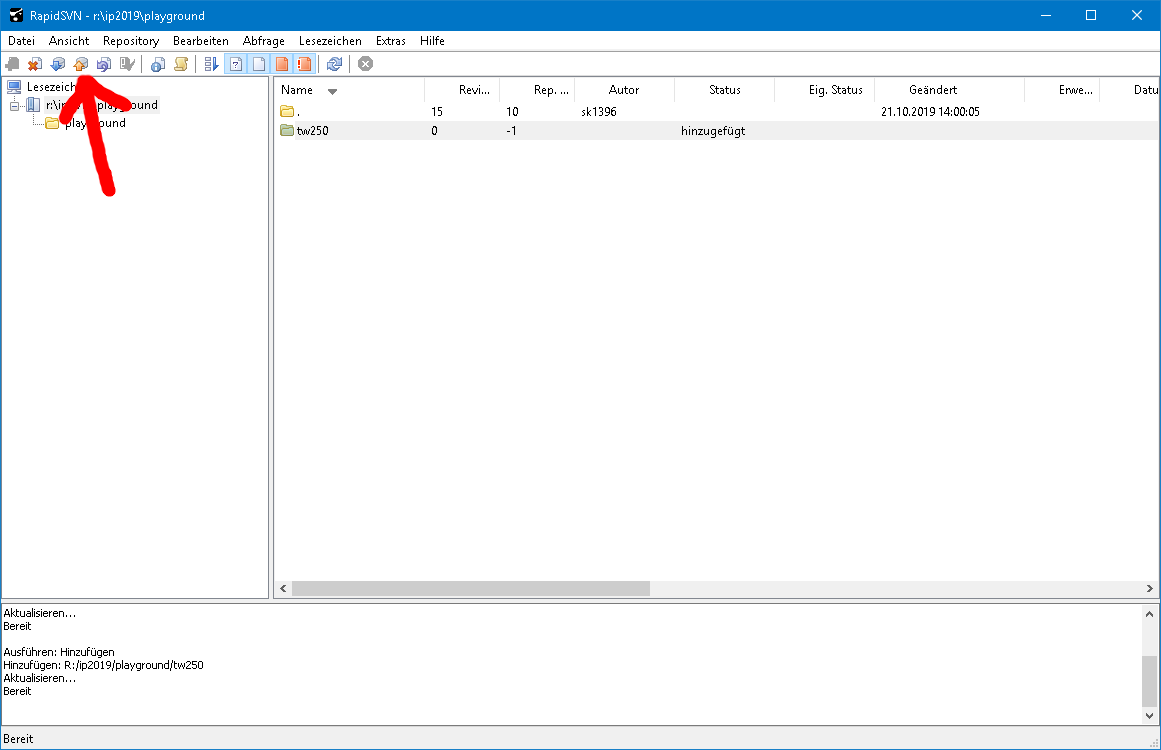
\includegraphics[width=\linewidth]{rapid10-2}
\end{center}

\clearpage

Dazu m�ssen wir einen Text eingeben, der unsere �nderungen beschreibt.

\begin{center}
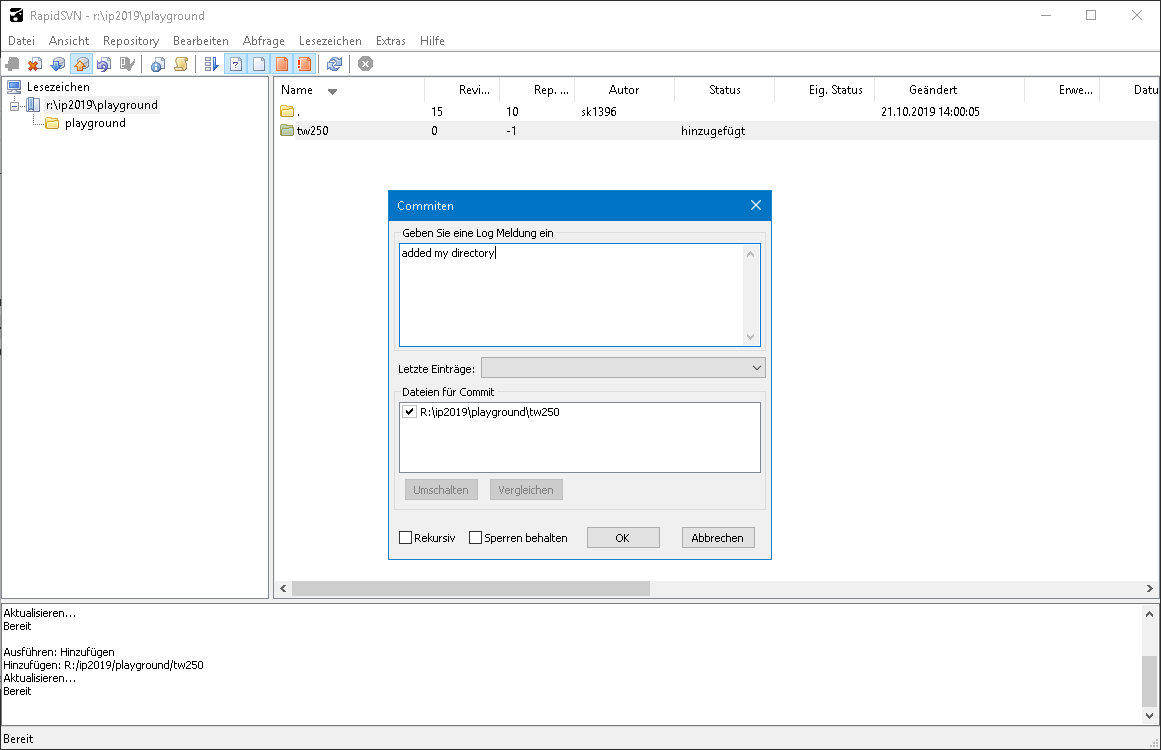
\includegraphics[width=\linewidth]{rapid11}
\end{center}

\clearpage

\section{Eine Datei commiten}

Wir k�nnen in unserem Ordner eine Datei erstellen.

\begin{center}
	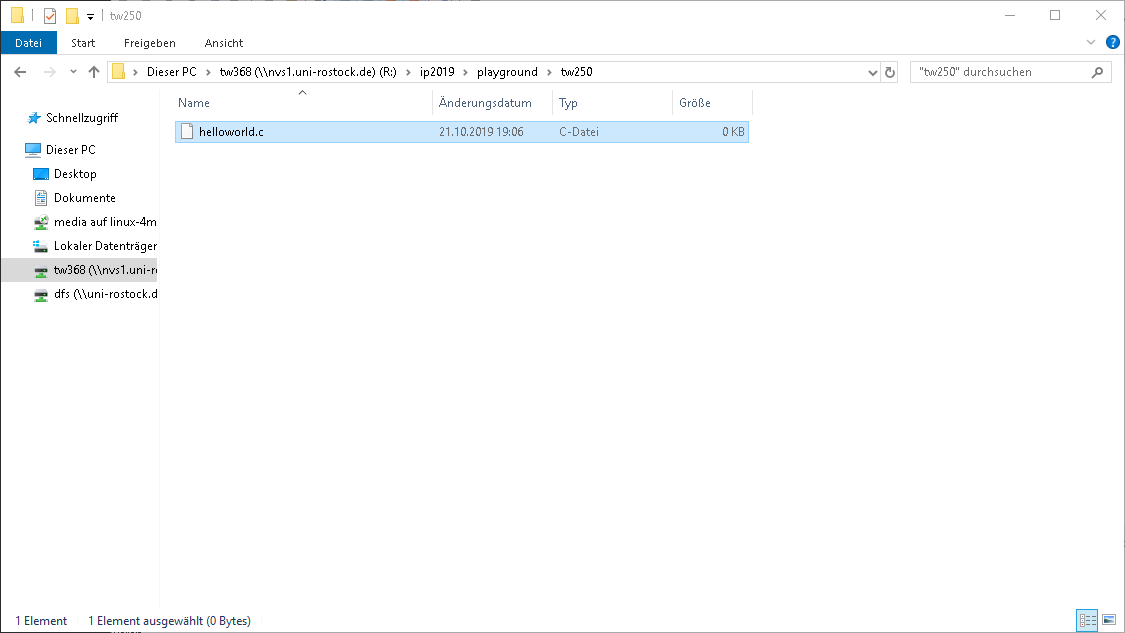
\includegraphics[width=\linewidth]{rapid12}
\end{center}

\clearpage

Sie ist zun�chst unversioniert.

\begin{center}
	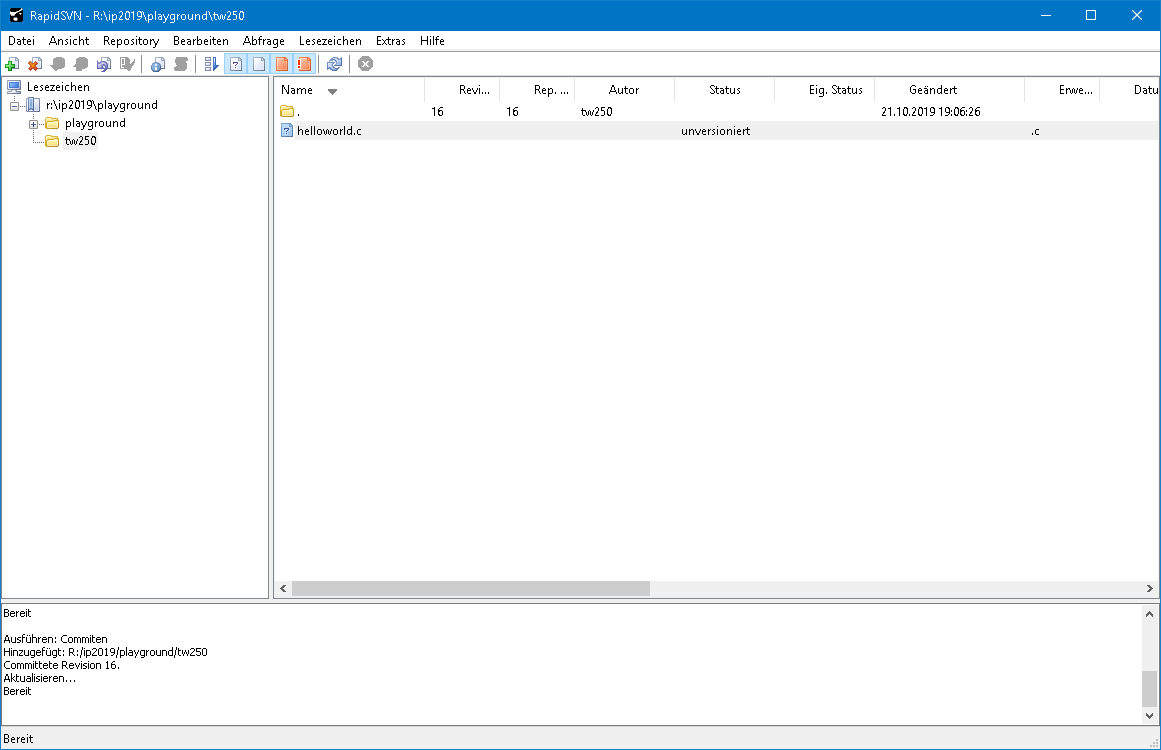
\includegraphics[width=\linewidth]{rapid13}
\end{center}

\clearpage

Um die Datei zu commiten, gehen wir vor wie bei einem Ordner. Erst die neue Datei hinzuf�gen...

\begin{center}
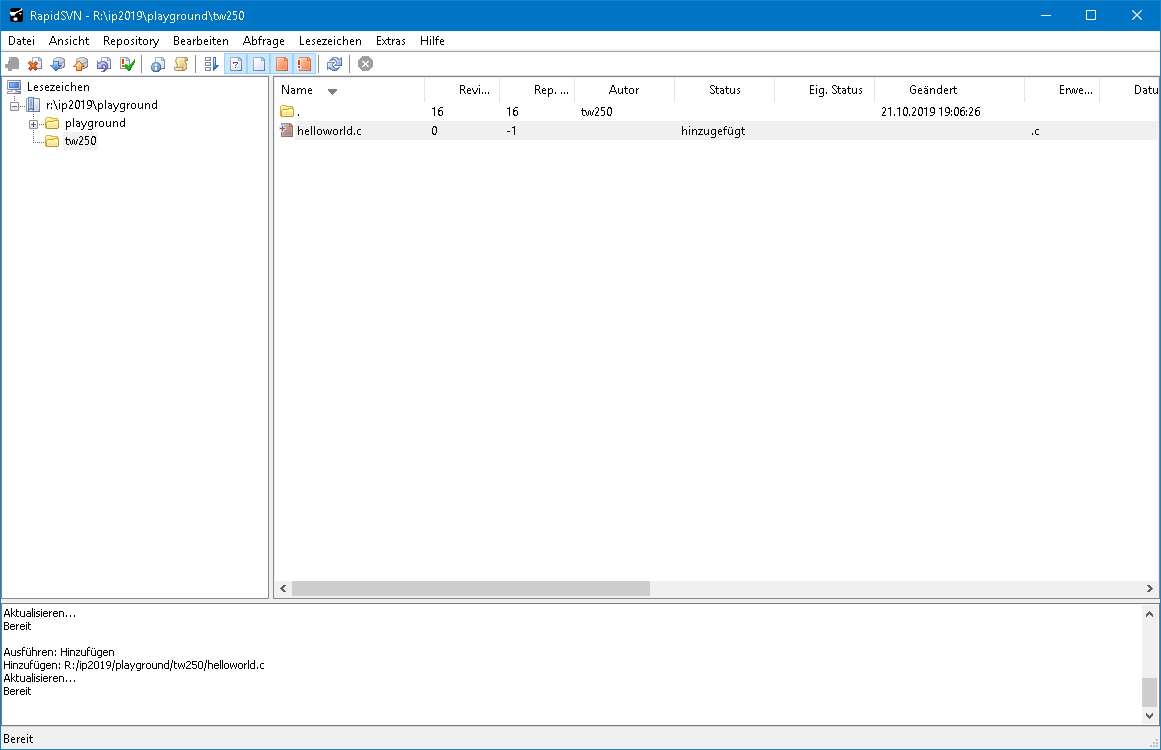
\includegraphics[width=\linewidth]{rapid14}
\end{center}

\clearpage

...dann commiten und dazu eine passende Commit Message angeben

\begin{center}
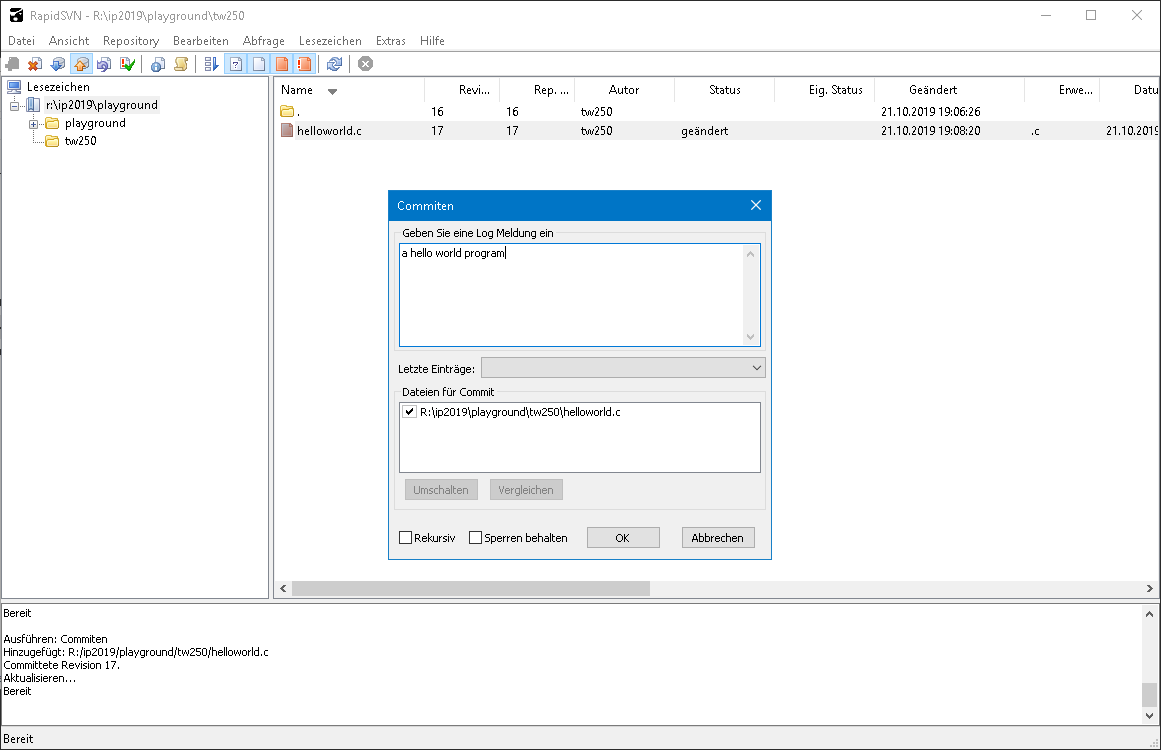
\includegraphics[width=\linewidth]{rapid15}
\end{center}

\clearpage

Fertig!

\begin{center}
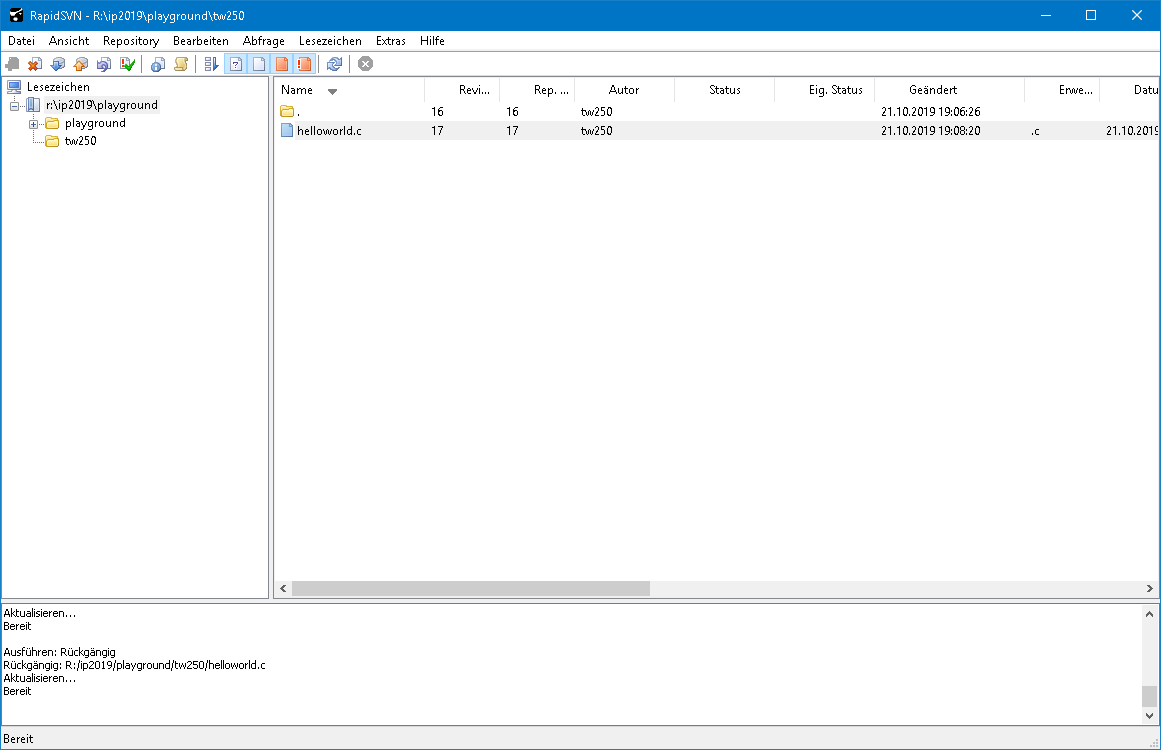
\includegraphics[width=\linewidth]{rapid16}
\end{center}

\clearpage

\section{�nderungen commiten}

Wenn der Inhalt einer Datei unter Versionsverwaltung ge�ndert wurde, wird sie als ge�ndert angezeigt.

\begin{center}
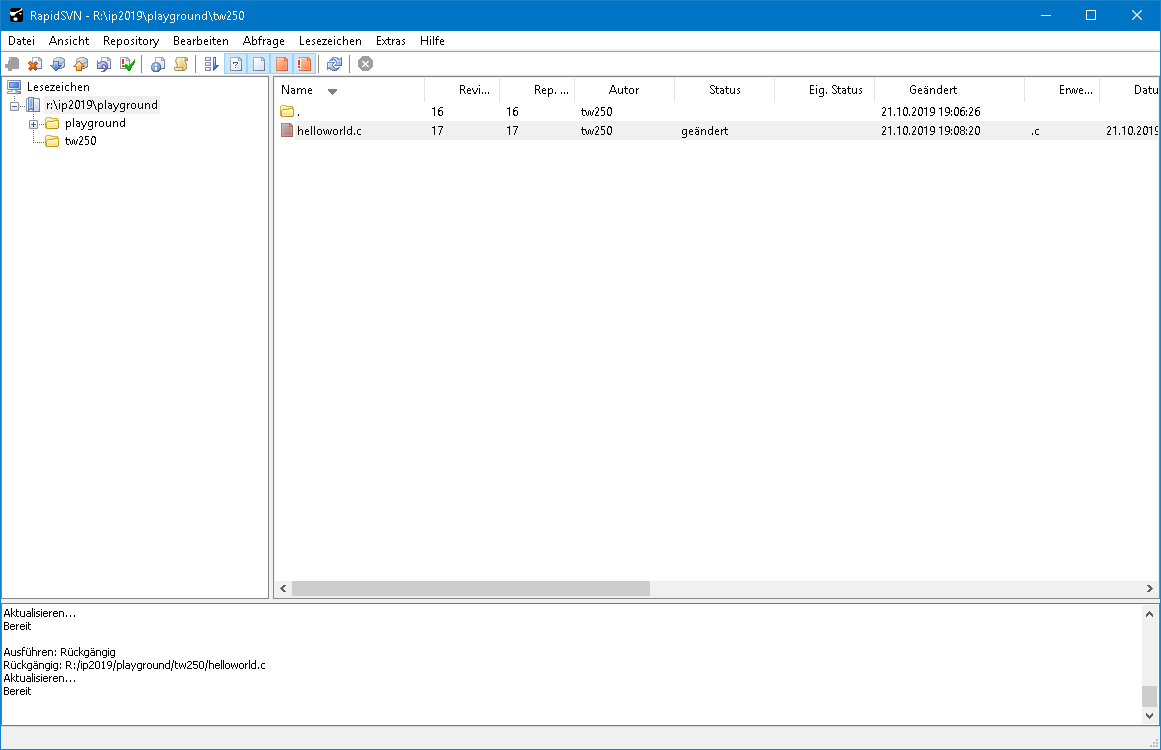
\includegraphics[width=\linewidth]{rapid17}
\end{center}

\clearpage

Wir k�nnen sie commiten und m�ssen dazu wieder eine passende Commit Message angeben.

\begin{center}
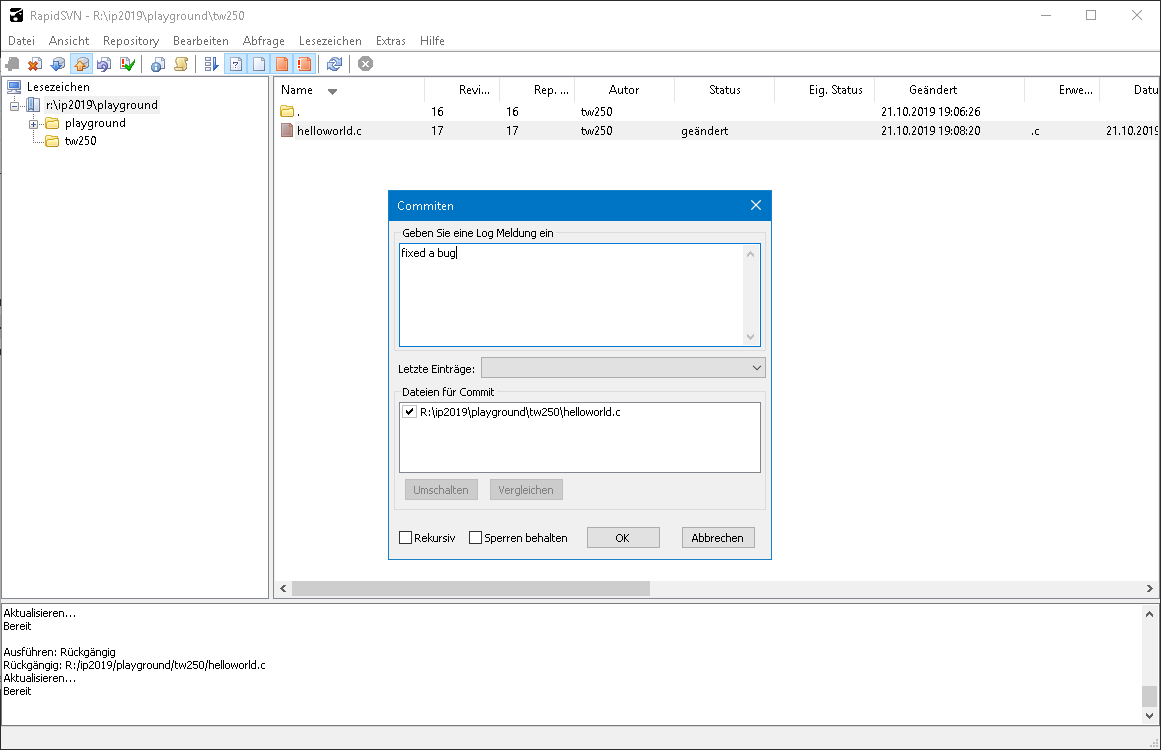
\includegraphics[width=\linewidth]{rapid18}
\end{center}

\clearpage

Nach dem Commit hat die Datei eine neue, h�here Versionsnummer.

\begin{center}
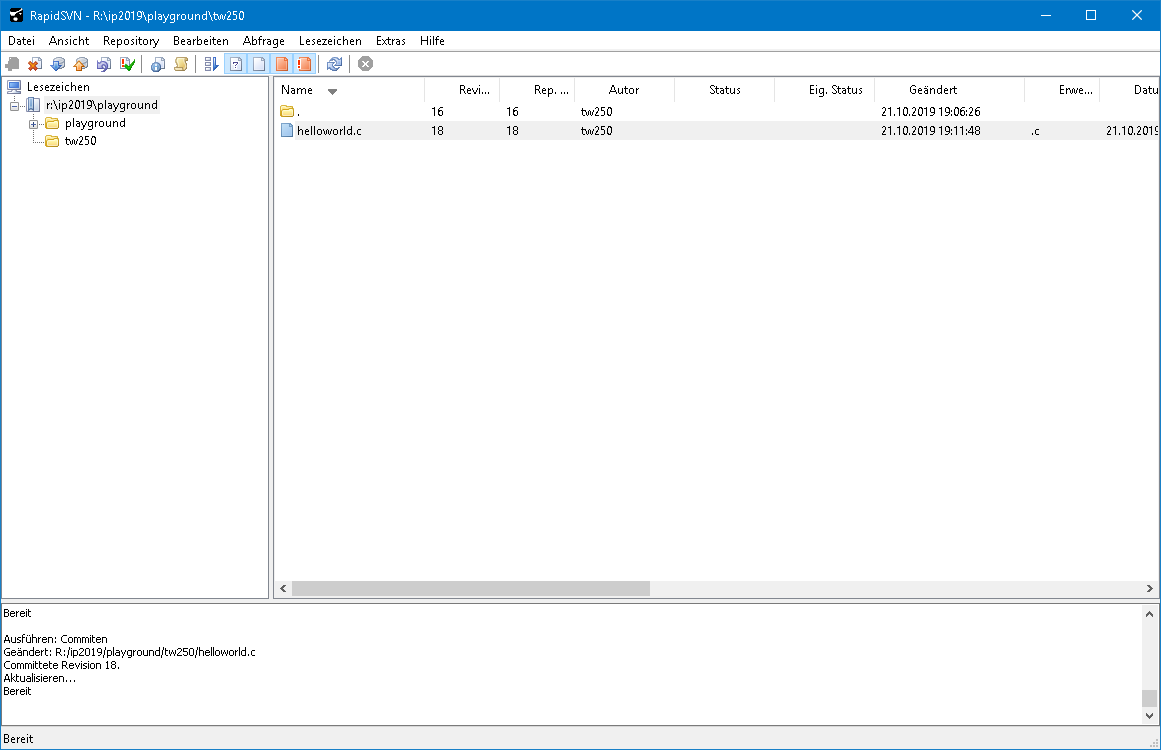
\includegraphics[width=\linewidth]{rapid19}
\end{center}

\clearpage

\section{Verlauf ansehen}

In dem Verlauf kann man alle Versionen der Datei sehen, die commitet wurden.

\begin{center}
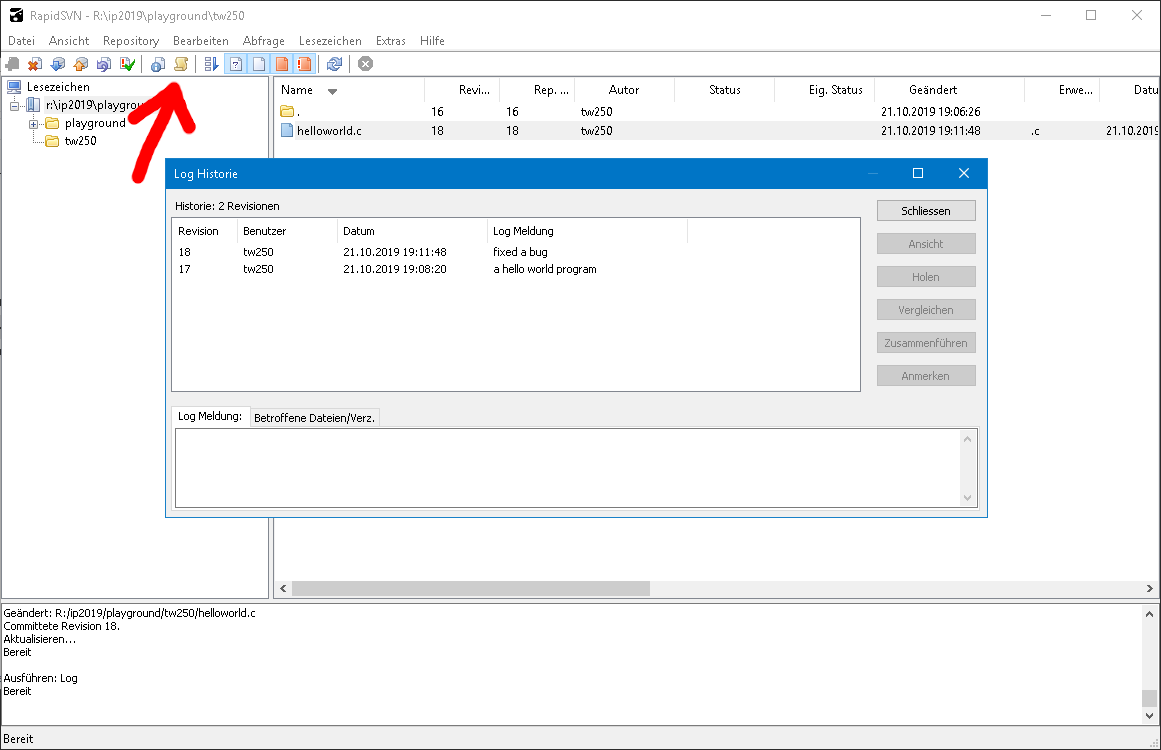
\includegraphics[width=\linewidth]{rapid20-2}
\end{center}

\clearpage

\section{Auf aktuellen Stand updaten}

Per Update kann man den aktuellen Stand vom Server holen.

\begin{center}
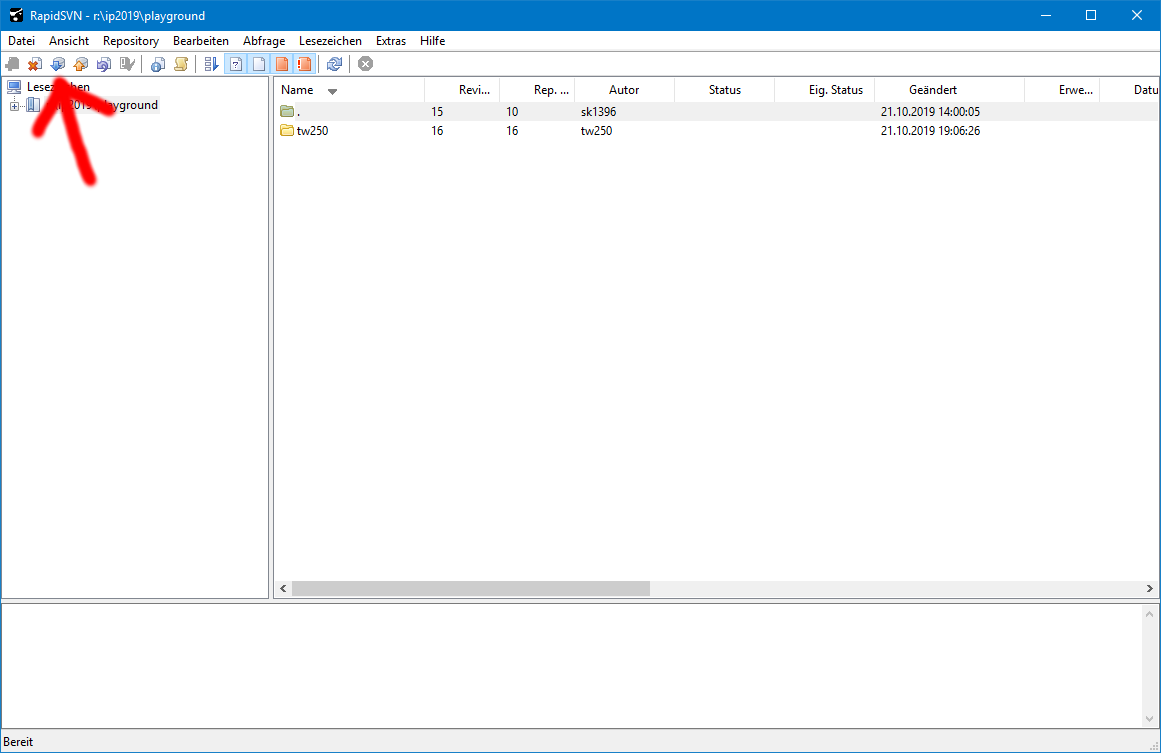
\includegraphics[width=\linewidth]{rapid21-2}
\end{center}

\end{document}